\chapter{Introduction}

Modern cameras -- both still-motion and video -- feature a high level of upgradability: lenses, filters and other accessories are all interchangeable, permitting finer control. As one of the most important components of the system, the image sensor plays a vital role in the composure of the final image. It dictates not only the output resolution, but also light sensitivity, colour representation, frame-rate and crop-factor. In spite of its significance, only a handful of expensive cinema and medium-format cameras include interchangeable sensors; even then, these components are proprietary. Upgrading the sensor in a mainstream camera requires the purchase of an entirely new system.

This paper details an FPGA-based sensor-agnostic interface which can be used to connect any image sensor to any image processor, thus providing the basis for a truly modular and upgradable camera system.

\section{A brief history of camera technology}

Modern cameras can trace their humble beginnings back to the camera obscura first described by ancient Chinese philosopher Mozi, who discovered an optical trick to pass light from an external scene through a hole and project it on a surface \cite{1_woolfson_2012}. In around 1816, French inventor Nicéphore Niépce managed to capture the first camera images using paper treated with silver chloride \cite{2_stokstad_cateforis_addiss_2005}. Continuing his work, Niépce's partner Louis Daguerre developed the first conventional camera using a simple lens to focus light onto a silver-coated copper plate \cite{3_harvard_library_preservation}.

\begin{figure}
  \centering
  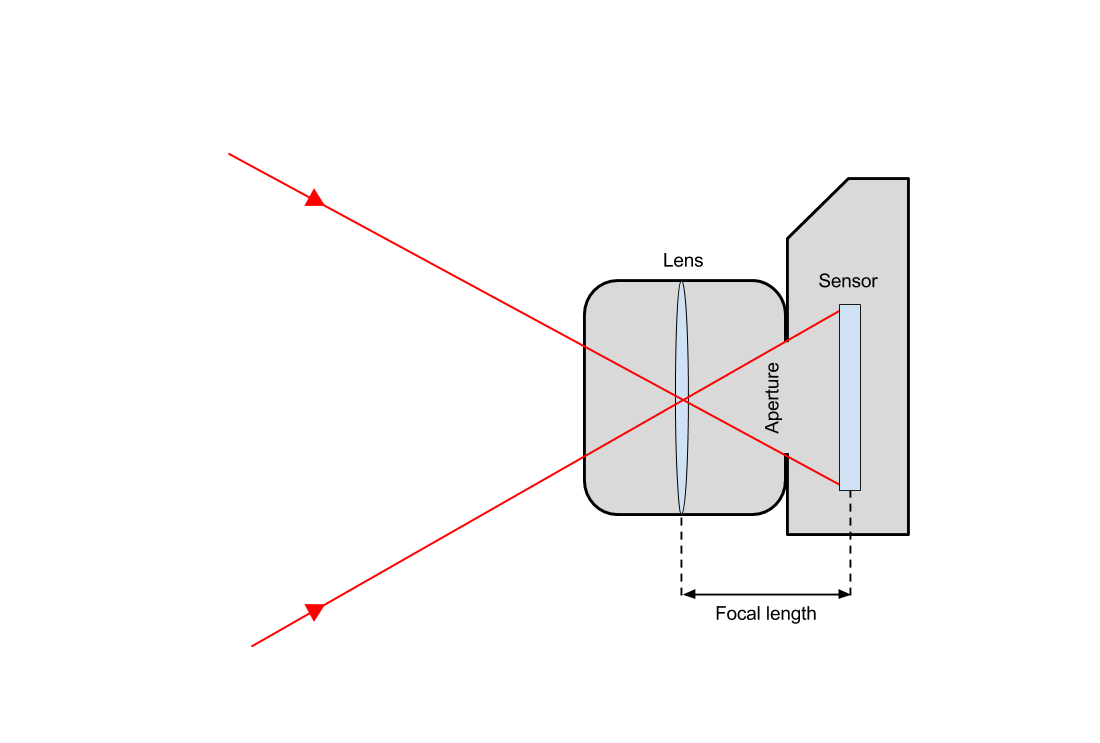
\includegraphics[width=1\textwidth]{./img/camera_physics_diagram.png}
  \caption{Light entering a camera and hitting sensor element}
  \label{fig:camera_physics_diagram}
\end{figure}

Figure \ref{fig:camera_physics_diagram} illustrates a very basic camera. Light from an external scene is focused by a lens and passed through an aperture hole where it is projected, inverted, onto a photosensitive surface for capture. The focal length dictates the distance between the optical centre of the lens and the sensor when the lens is focused to infinity \cite{4_pot_2010}. A shutter mechanism behind the aperture is used to control how much light hits the surface of the sensor, thus exposing the image. There are multiple ways to increase image exposure: expanding the aperture, holding the shutter open for longer, or increasing the ISO sensitivity of the sensor. Inversely, narrower apertures, shorter exposure times and lower sensitivities all decease the amount of light that hits the sensor, resulting in a darker image. 

Following the invention of the first transistor at Bell Laboratories in 1947, electronic devices could be dramatically reduced in size through the use of integrated circuits, paving the way for the start of the digital era \cite{5_computer_history_museum}. The first self-contained digital camera was developed by Steve Sasson of Eastman Kodak in 1975. Instead of using film, Sasson focused the light onto a state-of-the-art digital image sensor based on the first \gls{ccd} invented by Bell Laboratories scientists Willard Boyce and George Smith), the output of which was saved to a tape cassette for later viewing on a TV \cite{6_information_for_the_public,7_sasson_2007}.

Today, there are many different camera formats available -- one of the key differentiators being the area of the image sensor. A larger sensor can capture more light and thus the dynamic range is greatly increased, resulting in higher image quality \cite{8_chen_catrysse_el_gamal_wandell_2000}. This is true of both digital sensors, and their film counterparts.

\section{Motivation}

Professional camera systems are second-to-none when it comes to image quality and usability. The camera accessories market in Western Europe and the USA was worth \$1.7bn in 2006, a market which owed its existence to the modularity of modern cameras. With \$270 of accessories bought per \gls{dslr} camera on average, customisability is clearly an important feature \cite{9_understanding_and_solutions_2007}. Despite this, cameras lack customisability in one key area: IO expansion. Audio, video and storage interfaces are usually a fixed function of the camera's motherboard, and therefore non-interchangeable -- users must pre-empt their requirements in order to 'futureproof' their purchase. Inevitably these performance limits will be met; if a user wishes to step beyond these limits then an entirely new camera must be purchased. While some parts will undoubtedly be at the cutting edge of technology and require semi-frequent upgrades, other parts (camera bodies, audio amplifiers) may be technologically more mature and adhere to longer progression time-scales; thus it seems wasteful and costly to re-purchase these parts when buying a new camera system.

It is not the intent of this paper however, to suggest that the concept of an interchangeable camera sensor is entirely original -- a few high-end medium / large format cameras -- designed by Hasselblad, Phase One and Mayima -- exist which support interchangeable 'sensor backs' , however the interfaces are proprietary, thus limiting the user to a small handful of first-party options. Additionally, the prohibitively high price (upwards of \$10,000 at the time of writing) puts them far out of reach for the average professional photographer. Rather, the motivation of this project is to design an open standard for interchangeable sensors which can be freely implemented by anyone. In doing so, the basis for a truly modular and upgradable camera system is provided, with a broad range of applications including cinema, photography and computer vision. Figure \ref{fig:sensor_module} illustrates how this might work in practice. While idealistic, an open standard would benefit consumers by enabling new companies to gain a foothold serving smaller, more specialised markets which are too niche for established companies such as Nikon and Canon. Ultimately, this project aims to improve the camera selection available to consumers in the future by improving expandability options and fostering openness.

\begin{figure}
  \centering
  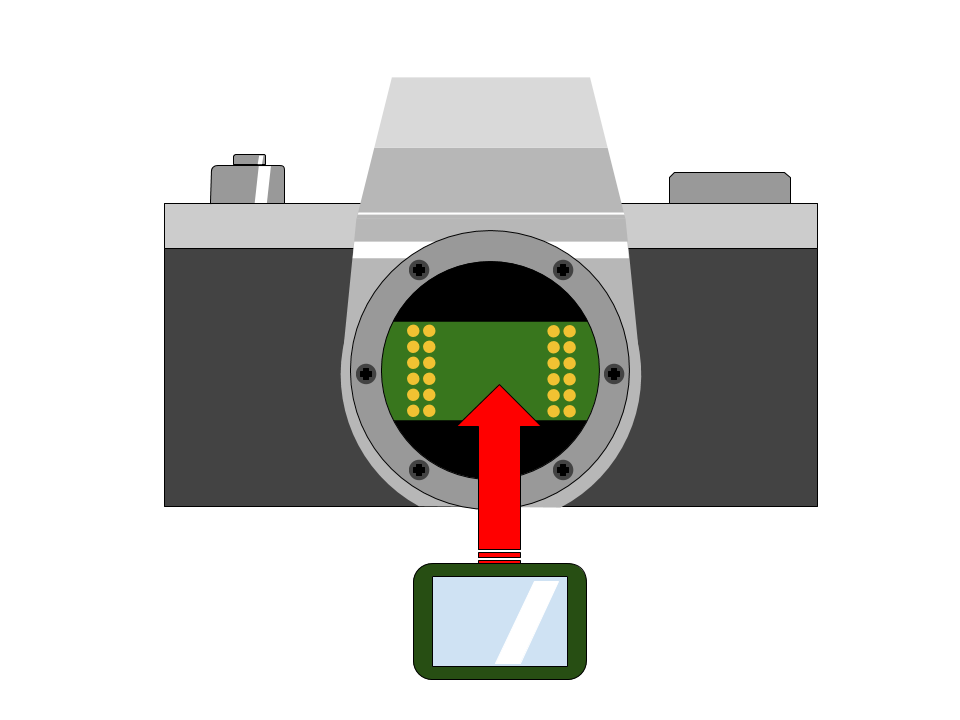
\includegraphics[width=1\textwidth]{./img/sensor_module.png}
  \caption{Inserting the sensor module into a camera}
  \label{fig:sensor_module}
\end{figure}



\section{Project testing platform}

The design of a full camera system is beyond the scope of this project, however an image sensor produced by OmniVision is used to capture real-world image data, providing a realistic test environment. \Glspl{fpga} are used extensively to set up a reconfigurable interface between the sensor and processor sides of the link, as well as generate test patterns for synthetic throughput and reliability tests. Given the main requirement of a sensor-agnostic interface is to work with a large range of sensors, there is a heavy emphasis on evaluating the system performance across several key metrics:

\begin{itemize}
  \item Reliability -- preserving signal integrity and ensuring low bit error rates for a stable and trustworthy system.
  \item Scalability -- transferring data across a wide range of resolutions and framerates to maintain a high level of expandability.
  \item Maximum throughput -- ensuring that the sensor interface does not bottleneck the system.
\end{itemize}

\subsection{Introduction to test system architecture}

The test system detailed in Figure \ref{fig:block_diagram_overview} is mainly based around the Zynq \gls{fpga} platform from Xilinx -- a programmable \gls{soc} with an embedded ARM core. \Glspl{fpga} are used instead of microcontrollers for several reasons, primarily because of the far greater flexibility of programmable logic, but also due to the high number of \gls{io} pins and throughput capabilities required to interface with high-resolution image sensors. \Glspl{fpga} are massively parallel and contain reconfigurable logic as well as multi-gigabit transceivers. Microcontrollers on the other hand, rely on fixed peripherals for a limited range of interface support; those which are not supported by the built-in peripherals must utilise bit-banging -- the process of using software to control the timing, synchronisation and state of \gls{io} ports to transmit or receive data. Microcontrollers simply lack the horsepower and resources to bit-bang a custom high-speed serial interface.

\begin{figure}
  \centering
  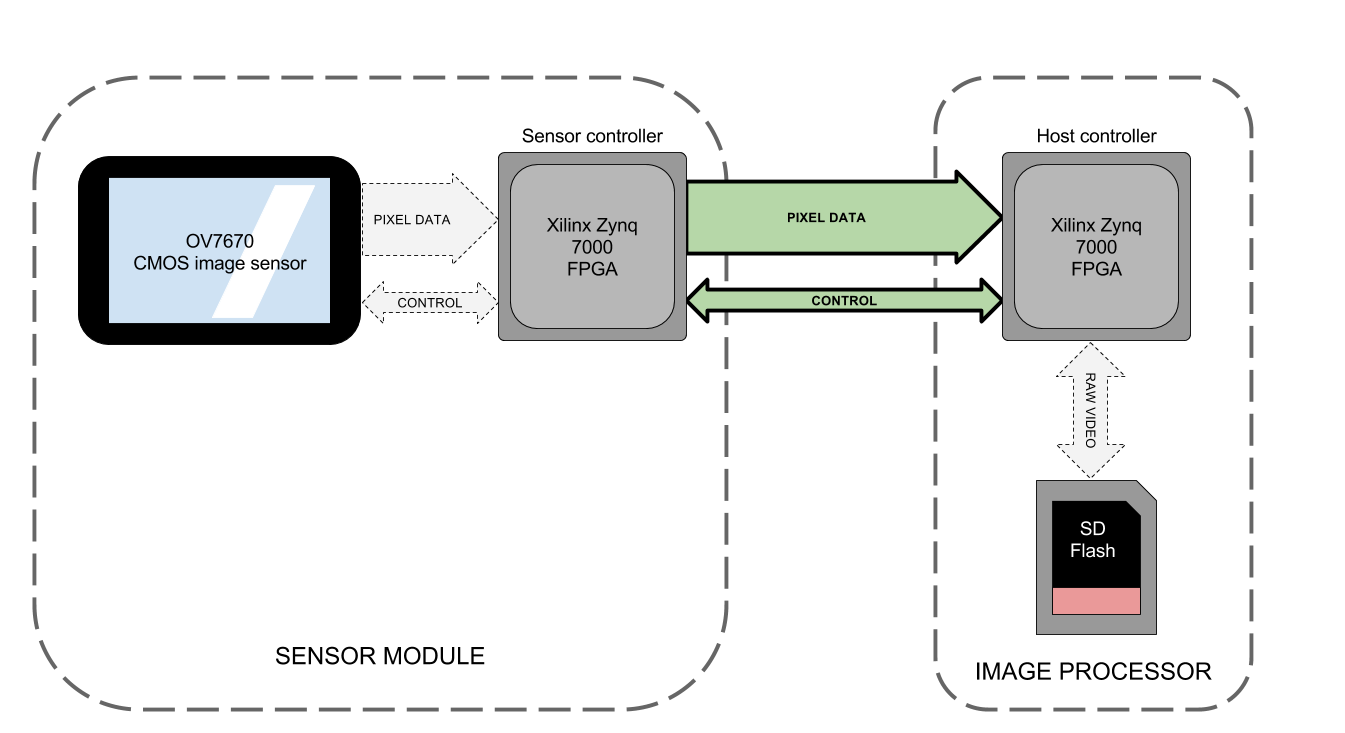
\includegraphics[width=1\textwidth]{./img/block_diagram_overview.png}
  \caption{Test system block diagram}
  \label{fig:block_diagram_overview}
\end{figure}

The system in Figure \ref{fig:block_diagram_overview} consists of an OmniVision OV7670 image sensor connected to a set of parallel inputs on a Xilinx Zynq 7000 \gls{fpga} acting as sensor controller. Pixel data is pulled from the sensor by the controller and placed into a \gls{ram} framebuffer where it can be retrieved by another part of the controller and transmitted across the interface. Optionally the controller can also generate a custom test pattern to be transmitted instead of the real sensor output for the purpose of system testing and benchmarking across a range of resolutions and framerates. These two components form the \textit{sensor module}, which is designed to be interchangeable with other sensor-controller pairs. The design of the interface highlighted in bold forms the main part of this project. 

On the master side of the interface is a second Zynq 7000 \gls{fpga} acting as the host controller. Pixel data going over the interface is received and decoded by the host before being stored in a framebuffer in \gls{ram}. The embedded ARM core inside the host forms the processing system, which takes each frame from \gls{ram} and serialises it into a RAW video stream in flash memory for playback on a computer. These components form the \textit{image processor}, which is capable of communicating with any connected \textit{sensor module}.

\subsection{Test system specification}

\begin{table}
  \centering
  \begin{tabular}{l | ll}
               & Minimum        & Maximum            \\
  \hline
  Resolution   & 640x480 (VGA) & 1920x1080 (1080p / FHD) \\
  Pixel depth  &                & 8-bit              \\
  Pixel format &                & Bayer RAW          \\
  Frame-rate   & 24p            & 60p                \\
  Throughput   &                & \SI{1}{\giga\bit\per\second}          
  \end{tabular}
  \caption{Sensor interface specification}
  \label{table:interface_specification}
\end{table}

The specifications in Table \ref{table:interface_specification} were decided after surveying best-selling cameras across several markets, consisting of cinema cameras, \glspl{dslr} and computer-vision / industrial cameras.